\documentclass[oneside]{book}
\usepackage[utf8]{inputenc}
\usepackage{makeidx}
\usepackage{graphicx}
\setcounter{tocdepth}{2}
\usepackage{hyperref}
\hypersetup{pdfborder={0 0 0},colorlinks=false}
\usepackage{verbatim}
\newenvironment{smallverbatim}{\endgraf\small\verbatim}{\endverbatim}
\newenvironment{tinyverbatim}{\endgraf\scriptsize\verbatim}{\endverbatim}
\pagestyle{plain}
\usepackage{float}
\usepackage{pdfpages}
\usepackage{listings}
\usepackage[paperwidth=21.59cm,paperheight=27.94cm]{geometry}
\usepackage{xcolor}


\author{Federico Campoli}
\title{PostgreSQL Database Administration \\ Volume 2 \\ Architecture}
\date{First edition, 2015, some rights reserved} 

\makeindex

\lstdefinestyle{pgsql}{
  belowcaptionskip=1\baselineskip,
  breaklines=true,
  frame=l,
  language=SQL,
  showstringspaces=false,
  basicstyle=\footnotesize\ttfamily,
  keywordstyle=\bfseries\color{green!40!black},
  commentstyle=\itshape\color{purple!40!black},
  identifierstyle=\color{blue},
  stringstyle=\color{orange},
  morekeywords={VACUUM, FULL, ANALYZE, TABLESPACE,SET,ALTER, SYSTEM}
}


\begin{document}
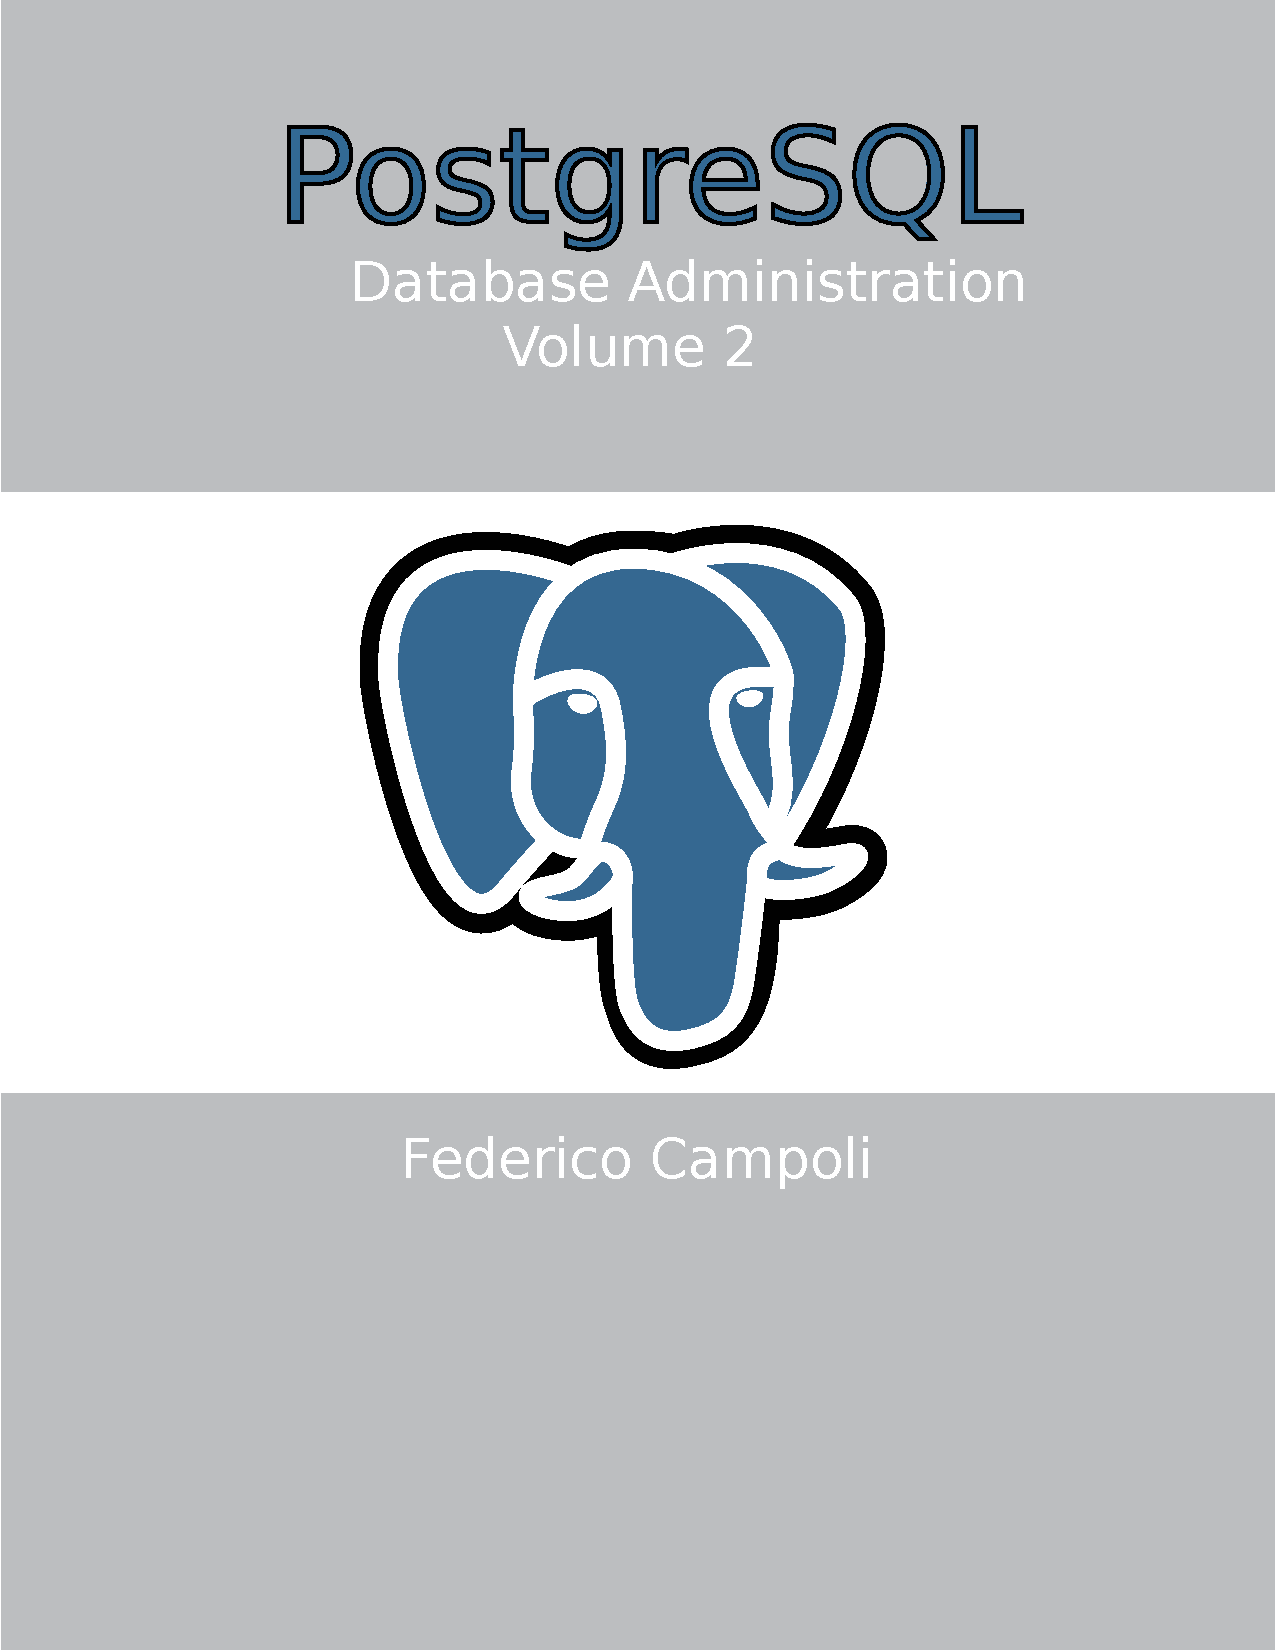
\includepdf{covers/cover_good.pdf}
\maketitle



\chapter*{License}
\begin{center}
 
\includegraphics{images/cc_logo.png}
\end{center}

The book is distributed under the terms of the Attribution-NonCommercial-ShareAlike 4.0 International 
License. To view a copy of this license, visit http://creativecommons.org/licenses/by-nc-sa/4.0/.\newline


You are free to:
\begin{itemize}
 
\item     Share — copy and redistribute the material in any medium or format
\item     Adapt — remix, transform, and build upon the material

\end{itemize}


Under the following terms:
\begin{itemize}
\item    Attribution — You must give appropriate credit, provide a link to the license, and indicate if 
changes were made. You may do so in any reasonable manner, but not in any way that suggests the licensor 
endorses you or your use.

\item    NonCommercial — You may not use the material for commercial purposes.

\item    ShareAlike — If you remix, transform, or build upon the material, you must distribute your 
contributions under the same license as the original.

\item    No additional restrictions — You may not apply legal terms or technological measures that legally 
restrict others from doing anything the license permits.

\end{itemize}

\chapter*{Copyright}
PostgreSQL Database Administration Volume 2 - Architecture\newline
Federico Campoli \copyright \space 2015 \newline
First edition\newline
%ISBN ???????????\newline



 



\chapter*{Preface}
Here we go again.


The github repository where I'm sharing the latex sources  is 
\href{https://github.com/the4thdoctor/pgdba\_books}{
https://github.com/the4thdoctor/pgdba\_books}.\newline


\section*{Intended audience}
Database administrators, System administrators, Developers

\section*{Book structure}
This book assumes the reader knows how to perform basic user operations such as
connecting to the database and creating tables.\newline

The book starts where the first volume ends, which reading is warmly suggested. After covering in depth the 
PostgreSQL architecture, there is a couple of chapters on the HA and disaster recovery. A final 
chapter is dedicated on the introduction of the performance tuning.\newline


\chapter*{Version and platform}
This book is based on PostgreSQL version 9.3 running on Debian GNU Linux 7.
References to older versions or different platforms are explicitly specified.

\chapter*{Thanks}
The beautiful cover has been made by \href{http://www.bonland.eu/}{Chiaretta e Bon }.\newline

\tableofcontents{}

\chapter{The cluster's architecture}
A PostgreSQL cluster is composed by a directory area initialised by init db and some processes 
accessing the data on disk and into a shared memory segment, the shared buffer. Those concepts were 
described briefly in the first volume. Now we'll see them in more details.

\section{Overview}



\chapter{The memory}
\label{ch:PGMEMORY}
The PostgreSQL memory at first sight looks simple. If compared with the complex structures implemented in 
the other DBMS to a careless reader could seem rudimentary. However, the memory and in particular the 
shared buffers implementation is complex and sophisticated. This chapter will dig down deep into the 
PostgreSQL's memory.

\section{The shared buffer}
The shared buffer is a segment allocated at cluster's startup. Its size is determined by the GUC parameter 
shared\_buffers and the size can be changed only restarting the cluster. The shared buffer is used 
to manage the data pages as seen in \ref{sec:CLUBACKEND}, which are called buffers when loaded in memory. 
Having a shared area into the RAM have also the beneficial effect of keeping the data near the CPU for 
rapid access, keeping in memory the important things and not everything. In the era of the \textit{in 
memory databases} this could seems quite obsolete but the truth is that the resources, and the money, are 
not infinite and the memory is not cheap.

\subsection{An horrible history}
\subsection{The clock sweep}
\subsection{The wal buffers}
\subsection{Memory context}

\section{The user memory}
\subsection{Work memory}
\subsection{Maintenance work memory}
\subsection{Temporary memory}

\section{Wrap up}
\chapter{The data area}


\chapter{The cluster in action}
\chapter{Point in time recovery}
\chapter{High availability}
\chapter{Performance Tuning}

\appendix

\listoffigures
\listoftables
\printindex{}
\end{document}
